\documentclass[12pt]{article}

\usepackage{graphicx}
\usepackage{fixltx2e}
\usepackage{color,soul}
\usepackage{placeins}
\usepackage{amsmath,amsfonts,amsthm} 

% fonts
\usepackage[scaled=0.92]{helvet}   % set Helvetica as the sans-serif font
\renewcommand{\rmdefault}{ptm}     % set Times as the default text font

% dmb: not mandatory, but i recommend you use mtpro for math fonts.
% there is a free version called mtprolite.

% \usepackage[amssymbols,subscriptcorrection,slantedGreek,nofontinfo]{mtpro2}

\usepackage[T1]{fontenc}
\usepackage{amsmath}
\usepackage{amsfonts}

% page numbers
\usepackage{fancyhdr}
\fancypagestyle{newstyle}{
\fancyhf{} % clear all header and footer fields
\fancyfoot[R]{\vspace{0.1in} \small \thepage}
\renewcommand{\headrulewidth}{0pt}
\renewcommand{\footrulewidth}{0pt}}
\pagestyle{newstyle}

% geometry of the page
\usepackage[top=1in, bottom=1in, left=1in, right=1in]{geometry}

% paragraph spacing
\setlength{\parindent}{0pt}
\setlength{\parskip}{2ex plus 0.4ex minus 0.2ex}

% useful packages
\usepackage{natbib}
\usepackage{epsfig}
\usepackage{url}
\usepackage{bm}


\begin{document}

\begin{center}
  \Large \textbf{The Meaning of Work and Productivity in Organizations} \\
  \vspace{0.1in}
  \large Stat/CS 8101: \textit{Applied Causality} \\
  \large Prof. David Blei \\
  \vspace{0.1in}
  \normalsize Natalie Carlson \\
  \today
\end{center}


\section{Introduction}

This course presented us with an exposure to causal inference dilemmas held by students across a variety of disciplines, the context of which may have at times been largely inscrutable to those of us coming from outside the area. I fear mine may have been no exception. I hoped, though, that the central question might prove universal: that is, what drives people to find their work to be meaningful, and does that sense of meaning in turn make them more productive workers. 

The context for my observational data comes from a 2012 survey, run at 571 microfinance branches nested within 19 organizations, across six states in India. At each branch, the branch manager and two loan officers were interviewed. The surveys were extensive, covering details on their activity breakdown, training, payment schemes, incentives, education and background, job enjoyment, and social measures, as well as details on the social service activities of the branch itself. The survey was intended to produce work on management practices and complementarities. The meaning-productivity relationship was something I noticed because it is a particular interest of mine.

The relationship in question I found striking: a clear, linear association between how meaningful the employees of a particular branch reported their work to be and the productivity of that branch. There is a great deal of literature in organizational behavior that suggests that employees who find meaning in their work will have higher levels of engagement, but no one had demonstrated a clear link to actual productivity. To be able to do so definitively would be of interest to both academics and practitioners.


\section{Previous Literature}

As previously mentioned, there is a large body of literature on meaning and the meaningfulness of work in the organizational behavior space. A perusal of Rosso et al.'s literature review (\citeyear{Rosso:10}), though, shows that the vast majority of this work focuses on the antecedents of and the psychological processes behind the generation of meaning, rather than its impacts. To the extent that prior work is concerned with the effects of meaningfulness in work, it is usually focused on engagement. Indeed, the seminal work of Kahn (\citeyear{Kahn:90}) on employee engagement places experienced meaningfulness among the three drivers of engagement, along with psychological safety and experienced availability.

In terms of quantitative evidence on meaning driving engagement, though, results are limited and mixed  \citep{Bailey:17}. Some of the most interesting work on meaningfulness in the workplace is qualitative in nature and derived from in-depth interviews. Pratt and Ashforth (\citeyear{Pratt:03}) emphasize that workplace meaningfulness is derived from community building, suggesting that two key elements are necessary for creating an organizational community: a family-like atmosphere, and a mission-driven focus with an emphasis on values. This values focus is echoed in Bailey and Madden's qualitative work on meaning (\citeyear{Bailey:16}), in which they find that employees' sense of meaning appears to be a deeply personal and individual phenomenon, focused on their work's wider contribution to society. They also delve deep into the symmetric construct of meaning\textit{less}ness, an event for which the most commonly cited cause was a conflict with the employee's personal value system.

The most closely related experimental evidence comes from an online experiment on prosocial incentives and productivity \citep{Tonin:15} . In this experiment, online workers performing a simple piece-rate data entry task were given an additional incentive: a donation to a charitable organization would be made as a result of their work. They found that this incentive increased task productivity by 13 percent, and that the effect was larger for those who were predisposed to prosocial motivation (those who reported volunteering in their free time). 

The fact that individual preferences and value systems may moderate the relationship between meaningfulness and productivity will play heavily into this analysis. Particularly, the observational dataset comprises microfinance organizations with different ownership types and identities: NGOs; for-profit firms known as NBFCs; and a subset of organizations which began as NGOs but morphed at some point into a for-profit model (hereafter referred to as switchers). The nature of these organization types may attract different employees and breed different cultures. Battilana and Dorado (\citeyear{Battilana:10}) describe microfinance institutions in general as hybrid organizations, combining both a "development logic" and a "banking logic". The switching companies in our sample, having been both non-profit and for-profit at different points in their life cycle, may fit this hybrid definition more than the others. 

\section{Observational Results and Causal Model}

Drawing on this literature and the measures available in the observational data, I have constructed an idealized version of a causal graph (Figure 1 in the Appendix). This model displays a unidirectional causal link from meaning to productivity, and three proposed factors that contribute independently to meaning: an interest in the type of work itself, a sense that the work contributes something positive to the community or world at large, and positive relationships in the workplace. In the observational data, these are operationalized largely from self-reported measures of the employees themselves. Table 1 models the right-hand side relationship in this causal graph, the link between meaning and productivity. The model is estimated using the following linear specification:

\begin{align} 
\begin{split}
Y_i = \alpha + \delta M_i + \beta X_i + \epsilon_i
\end{split}					
\end{align}

Here, $Y_i$ is the productivity measure, a branch level calculation: a ratio of the size of the loan portfolio that is not in default over the cost of labor and write-offs. $\delta$ is the causal effect of interest, and $M_i$ is an inverted measure of meaning: the average of the three branch employees' response to the prompt ``I sometimes feel my work is meaningless'' on a one-to-seven Likert scale.  $X_i$ is a vector of covariates, including indicator variables for the organization type, branch-level controls, and state- and MFI-level fixed effects. Including the full vector of control variables, as specified in Column (3), an increase of one point on the one-to-seven meaninglessness scale is estimated to be associated with about a tenth of a standard deviation reduction in productivity. Column (4) breaks down this estimated effect by organization-type subpopulation, following the specification:

\begin{align} 
\begin{split}
Y_i = \alpha + \delta_{NGO} M_i  [NGO=1]+ \delta_{NBFC} M_i  [NBFC=1] + \delta_{Switch} M_i  [Switch=1] \\
 +  \beta X_i + \epsilon_i
\end{split}					
\end{align}

The estimation of the coefficients within these subpopulations show that the average effect appears to be driven entirely by the NGO and Switching firms, with no estimated relationship for the for-profit firms. 

Table 2 models the left-hand side of the causal graph, the three independent drivers of meaning, following the specification:

\begin{align} 
\begin{split}
M_i = \alpha + \beta_1 I_i +  \beta_2 C_i  +  \beta_3 R_i +  \beta X_i + \epsilon_i
\end{split}					
\end{align}

In this model, $M_i$, the outcome variable, is once again the branch-level average of the meaninglessness question. $I_i$ refers to the additive scale for interest in the type of work, which corresponds to a question on why each employee took their current position. $C_i$, the term for community contribution, is operationalized as the mean Likert scale response to ``Our company contributes positively to the community'' and $R_i$, the term for relationships, is the analogous average for ``I like the people I work with.'' $X_i$ is a once again a vector of covariates and controls, including compensation. The estimated relationship between each of these measures and the outcome does not change substantially whether modeled separately (Columns 1-3) or together (Columns 4-5), which suggests that the causal model treating them as independent contributors is a reasonable approximation.

\section{The Crux of the Causality Issue}

While these linear regressions display a set of relationships in neat accordance with the causal model, the identification of the causal effect is quite easily challenged. One of the primary challenges could come in the form of a proposed reverse causal arrow from productivity to meaning:  that is, employees do not become more productive because they feel their work is meaningful, rather, they feel their work is meaningful precisely because their branch is efficient. Alternatively, one could propose an arrow from productivity to ``Our company contributes positively to the community''; similar to above, this would imply that employees might feel that their branch does more positive things for the world at large if it is productive. Finally, there could be any number of unobserved factors that might affect both perceived meaning and productivity; perhaps there is some latent trait that has a causal link to both constructs, and this back-door path explains the entire observed relationship.

Gelman and Imbens \citeyear{Gelman:13} make the distinction between reverse and forward causal questions, the former generally being of the form ``Why are X and Y associated?'' and the latter being the more easily tested ``What is the effect of X on Y?'' Here I will try to formulate the question in forward causal form: if one were to induce employees to find more meaning in their work, what would be the impact on productivity? This notion of inducing the proposed cause recalls the idea of the $do(.)$ operator \citep{Pearl:09}, a function of fixing a node of the causal graph at a particular value in order to isolate its impact on downstream variables. Our causal graph being impossible to entangle, and the key constructs being fuzzy and psychological in nature, I thought the best hope to approximate this was through a controlled experiment. 

\section{Experimental Design}

The goal of the experiment will be to replicate the notion of a $do(.)$ intervention on meaning, with the rationale being that if we can demonstrate the proposed causal effect in a separate sample, the interpretation of the observational data will become more plausible. To accomplish this, we will use online workers and manipulate the first two drivers of meaning on the causal graph in two separate experiments, with the intention of increasing the level of experienced meaningfulness and observing its effects on productivity.

The first experiment will push on the first lever we expect to drive meaning: interest in the work. We will recruit online workers via Amazon's Mechanical Turk and tell them we work with anonymous charitable organizations that require help with data entry. The task itself will remain common across conditions; it is the identity of the organization they are purportedly working for that we wish to manipulate. Those randomly assigned to the control condition will be shown a list of organizations -- anonymous, but with a note about their area of focus.  They will then be ``assigned'' to work for one of these organizations. The workers assigned to the treatment condition will instead be allowed to ``choose'' which organization they wish to work for. Again, the task itself will be identical. The outcome of interest will be the number of correct data entries in the allotted time (an indicator of productivity). To check that the manipulation had the intended effect, we will include a number of survey questions, including the perceived meaningfulness of the task. Therefore, a mediation analysis can be conducted, to confirm our proposed causal path. The experiment will conclude with a debrief that informs the workers of our minor deception and the purpose of our experiment.

The second experiment will instead manipulate the second driver of meaning -- the sense that the organization contributes positively to the world at large. In order to do this, we will take advantage of a useful phenomenon: charity effectiveness ratings. Similar to the control condition in the first experiment, each of the workers will be shown a list of organizations and told that they are assigned to one. In this case, however, an additional column will display the organization's effectiveness rating from an external source, such as CharityWatch. In the high effectiveness condition, the workers will be assigned to an organization with a high score, and in the low effectiveness condition, they will be given an organization with a relatively lower score. The subject area for this pair of organizations will be kept constant. The remainder of the experiment will proceed as above, and we will expect to see higher productivity for the individuals in the high effectiveness condition, mediated through an increased sense of meaning. 


\section{Conclusion and Future Directions}

If our experiment proves successful, the logical next step will be to examine the limitations of the causal relationship, and the contexts in which it does and does not hold. In the observational data, the relationship is observed only in the organizations that were not-for-profit at some point in their history; is the meaning-productivity association contingent on the prosocial content of the organization's mission? Or does it, perhaps, hold only for particular individuals who have a predisposition to being motivated by altruism? Can an experience of meaningfulness be induced through any other means? Pinning down these answers may prove useful to managers who struggle with employee engagement, academics that are interested in the psychological processes underlying the experience of meaningful work, and -- naturally -- journalists looking to write clickbait-y columns concerned with how best to enjoy one's job. Given the amount of time most people will spend in their chosen vocation, it may be comforting to know that finding an increased sense of meaning in those day-to-day tasks may also make them more effective.

\bibliographystyle{apalike}
\bibliography{references}

\section*{Appendix}

\begin{figure} [!h]
\centering
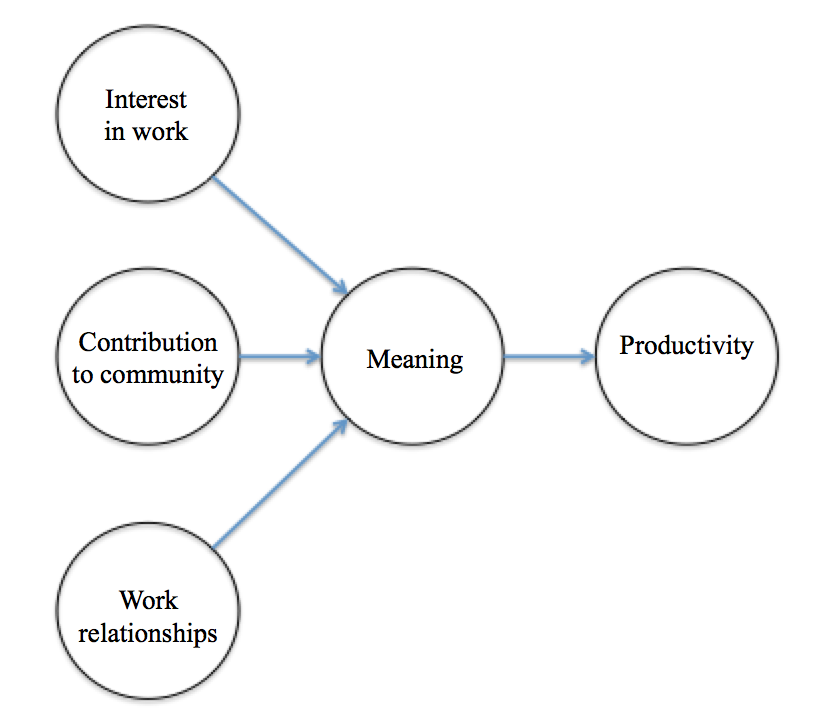
\includegraphics[scale=0.75]{causal_diagram}
\caption{Idealized causal graph}
\end{figure}

% Table created by stargazer v.5.2 by Marek Hlavac, Harvard University. E-mail: hlavac at fas.harvard.edu
\begin{table}[!htbp] \centering 
  \caption{Productivity Regressions} 
  \label{} 
\footnotesize 
\begin{tabular}{@{\extracolsep{5pt}}lcccc} 
\\[-1.8ex]\hline 
\hline \\[-1.8ex] 
 & \multicolumn{4}{c}{\textit{Dependent variable:}} \\ 
\cline{2-5} 
\\[-1.8ex] & \multicolumn{4}{c}{Productivity measure (standardized)} \\ 
\\[-1.8ex] & (1) & (2) & (3) & (4)\\ 
\hline \\[-1.8ex] 
 \textbf{`I sometimes feel my job is meaningless'} & \textbf{$-$0.14$^{**}$} & \textbf{$-$0.13$^{***}$} & \textbf{$-$0.09$^{**}$} &  \\ 
  & (0.06) & (0.05) & (0.04) &  \\ 
  `I sometimes feel my job is meaningless' x NGO &  &  &  & \textbf{$-$0.14$^{***}$} \\ 
  &  &  &  & (0.05) \\ 
  `I sometimes feel my job is meaningless' x NBFC &  &  &  & 0.01 \\ 
  &  &  &  & (0.03) \\ 
  `I sometimes feel my job is meaningless' x Switch &  &  &  & \textbf{$-$0.16$^{*}$} \\ 
  &  &  &  & (0.09) \\ 
  Always NGO &  & $-$0.42 & $-$0.01 & $-$0.09 \\ 
  &  & (0.32) & (0.02) & (0.26) \\ 
  Always NBFC &  & $-$0.13 & $-$0.04 & $-$0.54$^{**}$ \\ 
  &  & (0.25) & (0.04) & (0.27) \\ 
  Constant & 0.36$^{*}$ & 0.78$^{***}$ & 1.87$^{***}$ & 2.28$^{***}$ \\ 
  & (0.22) & (0.30) & (0.30) & (0.43) \\ 
 \hline \\[-1.8ex] 
Controls & No & Yes & Yes & Yes \\ 
State fixed effects & No & No & Yes & Yes \\ 
MFI fixed effects & No & No & Yes & Yes \\ 
\hline \\[-1.8ex] 
Observations & 423 & 396 & 396 & 396 \\ 
R$^{2}$ & 0.03 & 0.08 & 0.32 & 0.33 \\ 
\hline 
\hline \\[-1.8ex] 
\textit{Note: SEs clustered by MFI}  & \multicolumn{4}{r}{$^{*}$p$<$0.1; $^{**}$p$<$0.05; $^{***}$p$<$0.01} \\ 
\end{tabular} 
\end{table} 



% Table created by stargazer v.5.2 by Marek Hlavac, Harvard University. E-mail: hlavac at fas.harvard.edu
\begin{table}[!htbp] \centering 
  \caption{Drivers of Meaning} 
  \label{} 
\footnotesize 
\begin{tabular}{p{7cm}cccccc} 
\\[-1.8ex]\hline 
\hline \\[-1.8ex] 
 & \multicolumn{5}{c}{\textit{Dependent variable:}} \\ 
\cline{2-6} 
\\[-1.8ex] & \multicolumn{5}{c}{I sometimes feel my job is meaningless} \\ 
\\[-1.8ex] & (1) & (2) & (3) & (4) & (5)\\ 
\hline \\[-1.8ex] 
 \textbf{Took job because of interest in work} & \textbf{$-$0.10$^{***}$} &  &  & \textbf{$-$0.09$^{***}$} & \textbf{$-$0.09$^{***}$} \\ 
  & (0.03) &  &  & (0.03) & (0.02) \\ 
  \textbf{'Our company contributes positively to the community'} &  & \textbf{$-$0.28$^{***}$} &  & \textbf{$-$0.23$^{**}$} & \textbf{$-$0.24$^{**}$} \\ 
  &  & (0.10) &  & (0.10) & (0.10) \\ 
  \textbf{'I like the people I work with'} &  &  & \textbf{$-$0.24$^{**}$} & \textbf{$-$0.19$^{**}$} & \textbf{$-$0.21$^{**}$} \\ 
  &  &  & (0.09) & (0.10) & (0.09) \\ 
  BM total compensation (std) &  &  &  &  & 0.12 \\ 
  &  &  &  &  & (0.08) \\ 
  LO total compensation (std) &  &  &  &  & 0.06 \\ 
  &  &  &  &  & (0.10) \\ 
  Always NGO & 0.05 & $-$0.05 & $-$0.002 & 0.04 & 0.11 \\ 
  & (0.05) & (0.04) & (0.04) & (0.04) & (0.08) \\ 
  Always NBFC & 0.69$^{***}$ & 0.44$^{***}$ & 0.53$^{***}$ & 0.63$^{***}$ & 0.62$^{***}$ \\ 
  & (0.06) & (0.03) & (0.02) & (0.05) & (0.06) \\ 
  Constant & 1.87$^{***}$ & 3.11$^{***}$ & 2.70$^{***}$ & 4.46$^{***}$ & 4.67$^{***}$ \\ 
  & (0.37) & (0.81) & (0.53) & (0.82) & (0.89) \\ 
 \hline \\[-1.8ex] 
Controls & Yes & Yes & Yes & Yes & Yes \\ 
State fixed effects & Yes & Yes & Yes & Yes & Yes \\ 
MFI fixed effects & Yes & Yes & Yes & Yes & Yes \\ 
\hline \\[-1.8ex] 
Observations & 455 & 455 & 455 & 455 & 454 \\ 
R$^{2}$ & 0.20 & 0.19 & 0.17 & 0.23 & 0.24 \\ 
\hline 
\hline \\[-1.8ex] 
\textit{Note: SEs clustered by MFI}  & \multicolumn{5}{r}{$^{*}$p$<$0.1; $^{**}$p$<$0.05; $^{***}$p$<$0.01} \\ 
\end{tabular} 
\end{table} 




\end{document}
